\section{Introduction}
\label{sec:introduction}

\looseness=-1 World-model reinforcement learning enables sample-efficient learning in complex continuous control tasks \citep{wu2023daydreamer, hansen2024tdmpc2}. Continuous control demands temporal abstraction: locomotion with heterogeneous gait phases, contact-rich tasks with variable sensing rates, and multi-rate decision-making across planning horizons all require handling $\dt$ mismatches. TAWM \citep{nhu2025tawm} shows that conditioning a world model on step size $\dt$ yields consistent gains within TD-MPC2's MPC framework \citep{hansen2024tdmpc2}. Can the same $\dt$-conditioning bring temporal abstraction to imagination-based actor-critic methods like DreamerV3 \citep{hafner2025dreamerv3}, where policies are trained entirely in imagined rollouts?

We find that it cannot: every variable-rate configuration suffers substantial performance degradation. Through a factorial analysis on Walker Walk \citep{tassa2018dmcontrol}, we isolate the combination of a \emph{trained} $\dt$-embedding (a learned vector concatenated to the RSSM input at each imagination step; our implementation of $\dt$-conditioning) and multi-rate data exposure as the strongest predictor. This combination enables environment-dependent pathologies (reward prediction gaps in Walker Walk, or dynamics-model prior drift without measurable reward bias in Cheetah Run), which the critic internalizes as optimistic value estimates, a failure mode we term \emph{conditioning-induced value overestimation} (CIVO), analogous to delusional bias \citep{lu2018nondelusional} but model-induced rather than policy-class-induced. A normalized value-to-eval (NVE) diagnostic achieves perfect classification (AUROC${=}1.000$, $n{=}36$; Appendix~\ref{sec:appendix_sensitivity}).
\begin{figure*}[t]
\centering
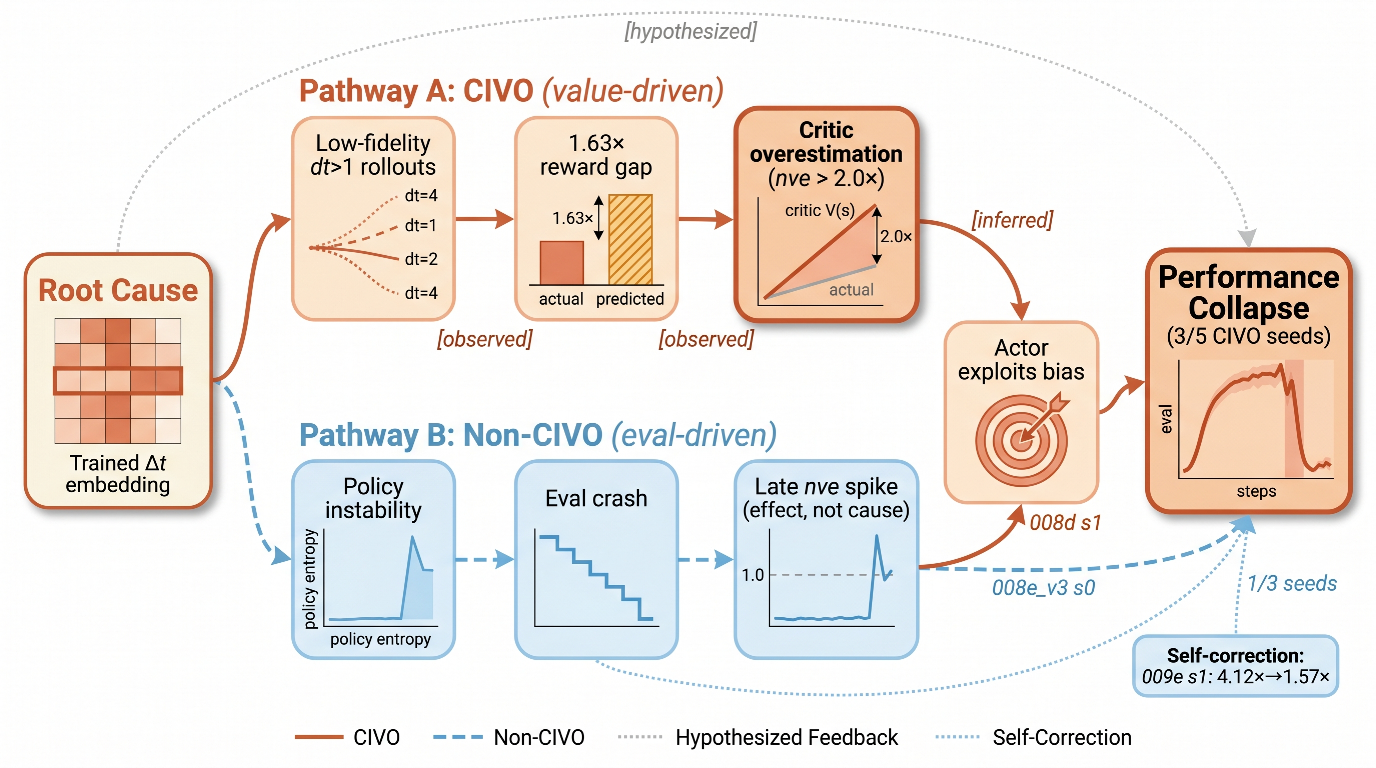
\includegraphics[width=\textwidth]{figures/paper/fig4_mechanism_diagram.pdf}
\caption{Proposed CIVO pathway (evidence levels annotated). The trained $\dt$-embedding enables asymmetric reward prediction fidelity (\textbf{observed}, ablation; Appendix~\ref{sec:appendix_analysis}), leading to optimistic critic values (\textbf{observed}, \S\ref{sec:f2}); actor exploitation of overestimated regions (\textbf{inferred} from entropy dynamics, Appendix~\ref{sec:civo_mechanism}) $\to$ reinforced state-distribution skew (\textbf{hypothesized}).}
\label{fig:civo_mechanism}
\end{figure*}

\looseness=-1 A four-level intervention hierarchy (gradient, output, representation, architecture) shows that most interventions fail to eliminate CIVO; only wide dual-critic (min-aggregation $+$ increased capacity) achieves partial prevention, though why this specific combination succeeds remains open. As world-model RL incorporates variable-rate decision-making, understanding when temporal conditioning fails is essential for the architectural design of variable-rate model-based RL.

\paragraph{Our contribution.}
\begin{enumerate}[nosep,leftmargin=*]
    \item \textbf{Failure mode identification.} We identify CIVO as specific to imagination-based actor-critic with temporal conditioning. Factorial analysis isolates trained $\dt$-embedding $+$ multi-rate exposure as jointly necessary for CIVO susceptibility; frozen and removed controls never trigger CIVO. The NVE diagnostic achieves perfect binary classification (AUROC${=}1.000$, $n{=}36$); cross-environment validation confirms specificity to moderate-complexity locomotion (\S\ref{sec:discussion}).
    \item \textbf{Structural barrier to remedy design.} A four-level intervention hierarchy (gradient, output, representation, architecture; 45 experiments) reveals that standard overestimation remedies are structurally ineffective in pure imagination: each class fails through a distinct mechanism (pathway redundancy, anchor co-drift, phase transitions, critic convergence in shared-data regimes), all traceable to the closed-loop constraint that the corrective signal originates from the overestimating model itself. Only wide dual-critic (min $+$ increased capacity) achieves partial prevention, the sole positive result across all tested approaches.
    \item \textbf{Mechanism analysis.} Frozen embeddings never trigger CIVO while trained embeddings frequently do ($p < 0.001$); this identifies embedding \emph{learning}, not conditioning architecture, as the causal factor. A $2{\times}2$ critic factorial dissects the architectural result: min-aggregation drives recovery, increased capacity enables prevention, and their combination is the minimum sufficient condition.
\end{enumerate}
